\chapter{タスク1：皮むき作業}
\label{ch:peeling}

本章では，第\ref{ch:introduction}章で設定した第一の研究課題である皮むき動作を扱う．
第\ref{ch:system}章で構築した3D点群モデル取得の共通基盤の上に，食材の皮むき動作を実現するための具体的なアルゴリズムと制御手法を述べる．
皮むき動作は，第1章で述べた「分析主導型」アプローチにおける「幾何学的な分析」の代表的な適用例であり，3D点群モデルから抽出した表面の法線や曲率といった幾何特徴に基づいて動作軌道を生成し，実行時には力覚フィードバックにより接触状態を維持するという，幾何と力学の統合が求められるタスクである．

本章で扱う皮むき動作は，一方のロボットアームがピーラーを把持し，他方のロボットアームが食材を支える双腕共同作業として構成される．
対象とする食材の表面形状には個体差が大きく，事前のCADモデルが利用できないため，その場で取得した3D点群モデルから動作計画に必要な幾何情報を抽出することが必須となる．
また，ピーラーの刃先を食材表面に沿って移動させる際には，単なる位置制御では点群計測誤差や表面の凹凸に対応できないため，力覚フィードバックによる接触力の維持が不可欠である．

以下では，まず皮むき動作の問題設定と全体手順を整理し，続いて幾何情報に基づく軌跡生成・分割・回転角計算の手法を述べ，さらにそれらを用いた動作計画と力覚フィードバック制御の統合について論じる．
最後に，複数種類の食材を用いた実機実験により，提案手法の有効性を検証する．

% 数字番号は，章・節タイトルではなく，上位節の中で説明する処理手順を表す．
% 本章では，第3章で得られた食材表面の3D点群モデルを入力とし，
% 点群取得，座標変換，多視点統合，平滑化，法線推定などの共通処理は繰り返して述べない．
% 符号は一括して冒頭に列挙せず，各処理の説明の中で必要に応じて定義する．

\section{皮むき動作の概要}  %% TODO整体的构成不太好
\label{sec:peeling_phase_overview}

本節では，本章で扱う皮むき動作の問題設定，作業全体の流れ，および使用する点群情報を整理する．
ここでは，アルゴリズムの詳細には入らず，本章全体の見取り図を与える．

\subsection{問題設定}
{
% TODO: 这两段说如何简化这个课题，真的可以么;这部分内容 感觉不像问题设定
皮むき動作では，一方のロボットアームがピーラーを把持し，他方のロボットアームが食材を支える双腕構成をとる．
本研究では調理器具として包丁ではなくピーラーを採用する．この選択には以下の二つの理由がある．

第一に，ピーラーの刃には切り込み深さを制限するリミッター（刃の間隔が固定する構造）が備わっている．
このリミッターにより，ピーラーを食材表面に一定の力で接触させ，目的の皮むき方向へ移動させるだけで，適切な深さの皮むきが実現される．
すなわち，包丁のように刃の角度や押し込み量を精密に制御する必要がなく，接触力の維持のみで皮むき動作が成立する．

第二に，ピーラーを用いることで，皮むき作業が「ピーラーを動かして一部の皮を剥く操作」と「食材を回転させて皮むき位置を変える操作」の二つに明確に分離される．
包丁では両手の協調動作が常時必要となるが，ピーラーではピーラー側の腕と食材固定側の腕の役割が時間的に独立するため，各操作の計画と制御が容易になる．

このような理由から，本タスクではピーラーを用い，対象とする食材の表面形状を $S$ とし，食材は串に固定されて回転軸 $\mathbf{v}_{\mathrm{rot}}$ 周りに回転できるものとする．
ピーラー側の腕は，食材表面に沿って刃先を移動させることで一部の皮を剥く「一回皮むき動作」を実行する．
食材固定側の腕は，一回皮むき動作が終了した後，未処理領域がピーラー側に来るように食材を回転させる「食材の回転操作」を実行する．
}

本章で解く問題は，以下のように整理できる．

\begin{enumerate}
  \item 食材表面の3D点群モデルから，ピーラーが倣うべき基準軌跡を生成する．
  \item 食材表面の法線変化に基づき，基準軌跡を実行しやすい複数の軌跡区間へ分割する．
  \item ピーラーと食材表面の接触を維持するため，力覚フィードバックを用いて刃先位置を補正する．
  \item 非皮領域の境界を検出し，次回の食材回転角を決定する．
  \item 皮むき動作と食材回転を反復し，終了条件を満たすまで皮むき範囲を拡大する．
\end{enumerate}

この問題設定は，人間がピーラーを用いて食材表面を一方向に剥き，その後食材を回して隣接領域を剥く手順を，双腕ロボット上で実現することに相当する．
人間は，食材の形状を視覚で捉えながらピーラーの刃先を表面に沿って滑らせ，適宜食材を回転させて未処理領域へと作業範囲を拡大していく．
本研究では，これらの機能を3D点群モデルに基づく幾何解析と力覚フィードバック制御の組み合わせにより工学的に実現する．

本タスクでは，以下の三つの仮定を置く．

\begin{enumerate}
  \item 対象食材は一つの代表的な中心軸を有し，その軸を基準として回転操作が可能であるものとする．この中心軸を食材の回転軸 $\mathbf{v}_{\mathrm{rot}}$ とし，皮むき軌跡の生成および皮むき後の食材回転に用いる．
  \item 食材は作業台 $\mathcal{P}_T$ 上に置かれており，作業台平面の法線ベクトル $\mathbf{n}_{\mathrm{ct}}$ は世界座標系の $z$ 軸方向と常に一致する．
  \item 一回皮むき動作で剥かれる領域は，幅が一定の矩形形状となる．すなわち，剥かれた皮の幅は軌跡上の全位置で同一である．
\end{enumerate}

これらの仮定のもとで，提案手法は食材の個体差（形状，大きさ，表面曲率）に対して適応的に皮むき動作を生成することを目指す．

\subsection{皮むき動作の全体手順}

皮むき作業は，「一回皮むき動作」と「食材の回転操作」の反復として構成する．
ここで，一回皮むき動作とは，ピーラーを食材表面に接触させ，あらかじめ生成した軌跡に沿って移動させる処理である．
食材の回転操作とは，一回皮むき動作の後に，次に剥くべき領域がピーラー側へ向くように食材を回転させる処理である．

全体手順は以下のように整理できる（図\ref{fig:peeling_sequence}）．

\begin{enumerate}
  \item 第3章の手順により得られた食材表面のRGB点群 $P_{\mathrm{all}}$ を入力する．
  \item 食材の回転軸 $\mathbf{v}_{\mathrm{rot}}$ を含む断面抽出平面を用いて，食材断面を抽出する．
  \item 断面輪郭から，到達困難な下側部分を除去し，到達可能な基準軌跡 $L$ を得る．
  \item 基準軌跡 $L$ 上の法線変化を用いて，軌跡を複数のセグメント $s_j$ に分割する．
  \item 各セグメントに沿ってピーラーを移動させ，力覚フィードバックにより接触力を維持する（一回皮むき動作の実行）．
  \item 一回皮むき動作の後，RGB情報を用いて非皮領域とその境界 $L_p$ を抽出する．
  \item 境界近傍の平均法線 $\mathbf{n}_{\mathrm{avg}}$ から，食材の回転角 $\alpha$ を計算する．
  \item 食材を $\mathbf{v}_{\mathrm{rot}}$ 周りに $\alpha$ だけ回転させ，次の一回皮むき動作へ移る．
  \item 終了判定を満たすまで，必要に応じて点群を再取得しながら，ステップ2〜8を反復する．
\end{enumerate}

% TODO：图的位置不对
% \begin{figure}[t]
%     \centering
%     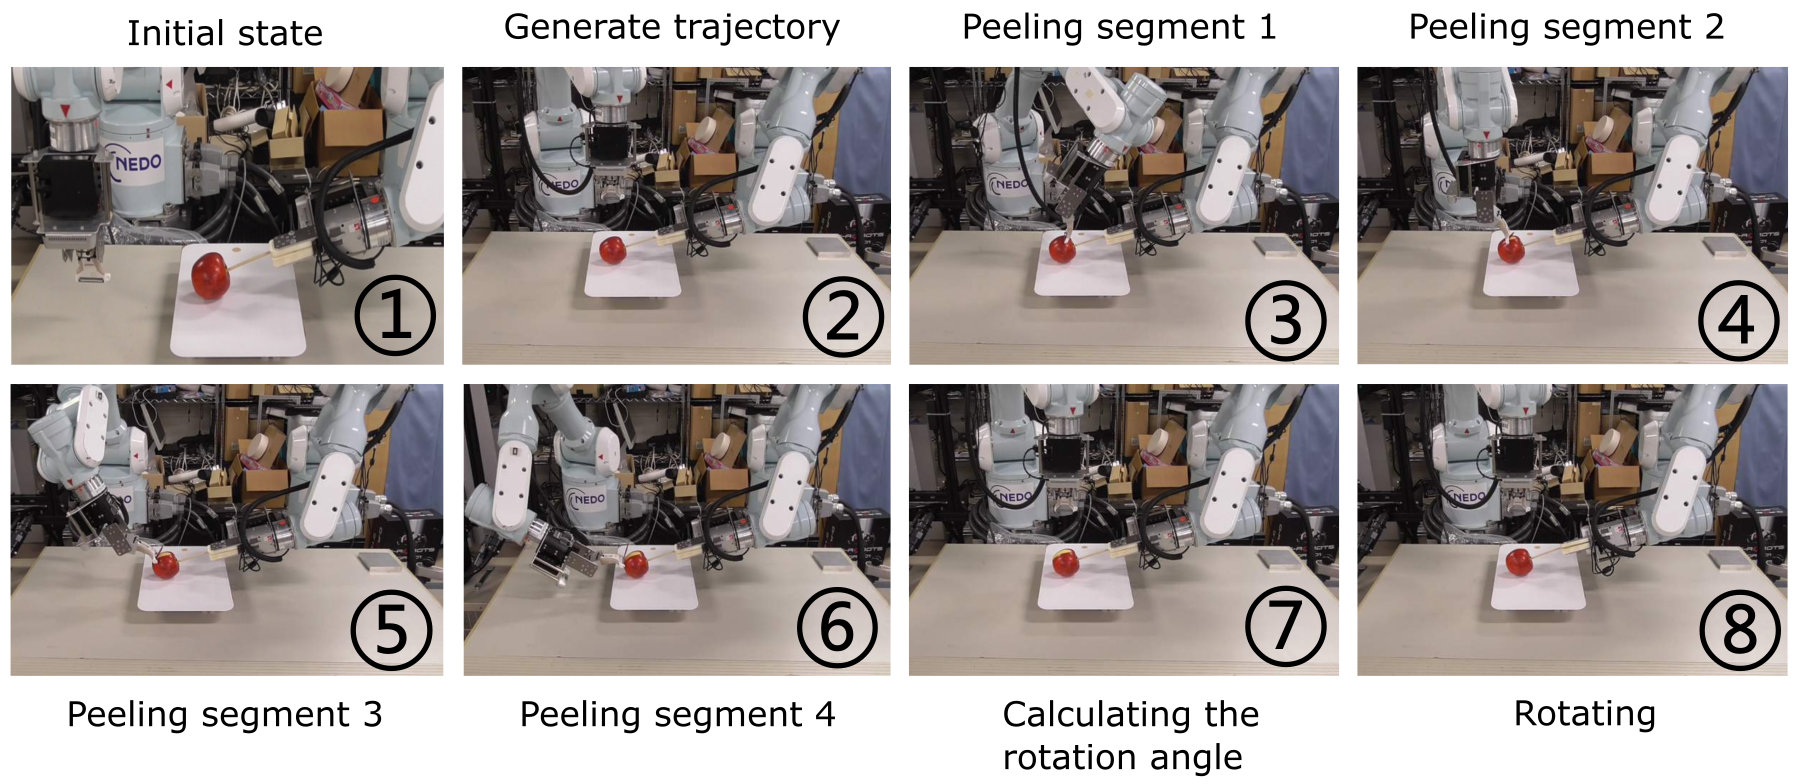
\includegraphics[width=0.7\textwidth]{fig/chp_peeling/sequence.png}
%     \caption{提案する皮むき手法の全体シーケンス．終了条件を満たさなければ，Step~8 の後 Step~2 へ戻る．}
%     \label{fig:ch4_sequence}
% \end{figure}

ここでは，$P_{\mathrm{all}}$，$L$，$s_j$，$L_p$，$\alpha$ などの符号を，全体手順の中で必要な順に導入する．
以降の節では，これらの量をどのように求め，ロボットの動作へ接続するかを述べる．

\subsection{使用する点群情報}

本章で使用する点群情報は，第3章で述べた3Dモデル取得手順により得られたものである．
具体的には，以下の情報を用いる．

\begin{enumerate}
  \item \textbf{食材表面点群 $P_{\mathrm{all}}$} \\
  食材全体の外表面を表すRGB点群であり，基準軌跡の抽出，非皮領域の検出，終了判定に用いる．
  $P_{\mathrm{all}}$ は，第3章の共通処理パイプライン（多視点撮影，座標変換，統合，ダウンサンプリング，外れ値除去，クラスタリング，MLS平滑化）を経て得られたものであり，各点は3次元座標 $(x, y, z)$，RGB色情報，および法線ベクトル $\mathbf{n}_i$ を有する．
  法線ベクトルはMLS（Moving Least Squares）法\cite{PCL-MLS}により計算され，食材の外側を向くよう統一されている．

  \item \textbf{表面点 $\mathbf{p}_i$ と法線 $\mathbf{n}_i$} \\
  点群中の各点を $\mathbf{p}_i$，その法線を $\mathbf{n}_i$ とする．
  法線情報は，軌跡分割，ピーラー姿勢の決定，食材回転角の計算に用いる．

  \item \textbf{RGB情報} \\
  皮と非皮領域の色差を利用し，非皮領域および境界 $L_p$ を抽出するために用いる．
  具体的には，RGB色空間からHSV色空間への変換を行い，事前に定義されたHSV範囲に基づいて非皮領域を識別する．

  \item \textbf{作業台平面と回転軸} \\
  作業台平面を $\mathcal{P}_T$，その法線を $\mathbf{n}_{\mathrm{ct}}$ とする．
  作業台平面の法線 $\mathbf{n}_{\mathrm{ct}}$ は，第3章で述べたRANSAC法\cite{PCL-RANSAC}により点群から自動抽出される．
  また，食材の回転軸を $\mathbf{v}_{\mathrm{rot}}$ とする．これは食材の中心軸として人手により指定される．
  これらは，断面抽出と食材回転を記述する基準として用いる．
\end{enumerate}

これらの点群情報は，いずれも第3章の共通処理パイプラインを経て取得されるため，本章では個々の取得手順を繰り返し述べることはせず，必要に応じて第3章の該当節を参照する形で記述を進める．

\section{幾何情報による皮むき動作の分析}
\label{sec:peeling_phase_geo}

本節では，食材表面の3D点群モデルから，皮むき動作に必要な幾何情報を抽出する方法を述べる．
具体的には，断面輪郭に基づく基準軌跡の抽出，表面法線による軌跡分割，および非皮領域境界に基づく回転角の計算を扱う．
これらの処理は，本論文の「分析主導型」アプローチにおける「幾何学的な分析」の中核をなすものであり，物理的な接触を伴わない事前の計算段階で，食材形状に適応した動作パラメータを導出することを目的とする．

\subsection{軌跡の抽出}
\label{sec:peeling_trajectory}

一回皮むき動作では，ピーラーの刃先が食材表面に沿って移動する必要がある．
食材の形状は個体ごとに異なるため，あらかじめ固定された軌跡を用いることはできず，その場で取得した食材表面点群から基準軌跡を抽出する必要がある．
仮定より，食材は回転軸 $\mathbf{v}_{\mathrm{rot}}$ 周りのみに回転するため，各回の皮むきで最大の剥き幅を得るには，刃先を表面に沿って，かつ回転軸 $\mathbf{v}_{\mathrm{rot}}$ に「平行」に滑らせるのが最も単純かつ効果的な方法である．

そこで，以下の手順により基準軌跡を生成する．

\subsubsection{断面抽出平面1による断面輪郭の抽出}

まず，食材の回転軸 $\mathbf{v}_{\mathrm{rot}}$ を含み，作業台平面 $\mathcal{P}_T$ に垂直な平面を断面抽出平面 $\mathcal{P}_{c1}$ として定義する．
$\mathcal{P}_{c1}$ は，食材の回転軸に沿った鉛直断面を切り出すための平面である．

この断面抽出平面 $\mathcal{P}_{c1}$ により食材形状 $\mathrm{S}$ を切断し，断面領域 $A_c$ と断面輪郭 $L_c$ を得る．
実際の処理では，食材表面点群 $P_{\mathrm{all}}$ から $\mathcal{P}_{c1}$ に近い点（点と平面の距離が閾値以内の点）を抽出し，それらを断面輪郭 $L_c$ の離散表現とする．
今回の実験では，この閾値を0.3\,mmとした．この値は，使用する点群の密度に依存して定められる．

\subsubsection{到達可能軌跡の抽出}

断面輪郭 $L_c$ の全体がロボットにとって実行可能な軌跡になるわけではない．
食材の下側部分，すなわち作業台に近い領域は，作業台やロボットアーム，串固定部との干渉により到達が困難である．
そのため，到達可能性を判定するための到達可能性判定平面2 $\mathcal{P}_{c2}$ を導入し，$L_c$ のうち到達困難な部分を除去する．

$\mathcal{P}_{c2}$ は，回転軸 $\mathbf{v}_{\mathrm{rot}}$ を通り，その法線 $\mathbf{n}_{c2}$ が以下の条件を満たす平面として定義される．

\begin{align}
  \mathbf{n}_{c2} &= \mathbf{r} \times \mathbf{n}_p \label{eq:peeling_cut_plane_2}
\end{align}

ここで，$\mathbf{n}_p$ は以下の条件を満たすベクトルである．

\begin{equation}
  \mathbf{n}_p \cdot \mathbf{n}_{\mathrm{ct}} = 0,\quad
  \mathbf{n}_p \cdot \mathbf{v}_{\mathrm{rot}} = 0,\quad
  \mathbf{n}_p \cdot \mathbf{n}_{\mathrm{ct}} \ge 0
\end{equation}

すなわち，$\mathbf{n}_p$ は $\mathcal{P}_{c2}$ 上にあり，回転軸 $\mathbf{v}_{\mathrm{rot}}$ と作業台平面の法線 $\mathbf{n}_{\mathrm{ct}}$ の両方に直交するベクトルである．

断面輪郭 $L_c$ の各点 $\mathbf{p}_i$ に対して，以下の条件を満たす点を到達困難点として除去する．

\begin{equation}
  \mathbf{v}_i \cdot \mathbf{n}_{c2} > 0
  \label{eq:peeling_point_removal}
\end{equation}

ここで，$\mathbf{v}_i$ は世界座標系の原点から点群 $P_{\mathrm{all}}$ 中の点 $\mathbf{p}_i$ へ向かうベクトルである．
除去後に残った輪郭を，到達可能な基準軌跡 $L$ とする．
基準軌跡 $L$ の点群を $P_L$ と表記する．
この処理を図\ref{fig:peeling_trajectory}に示す．

\begin{figure}[t]
    \centering
    \begin{subfigure}[t]{.45\textwidth}
    	\centering
    	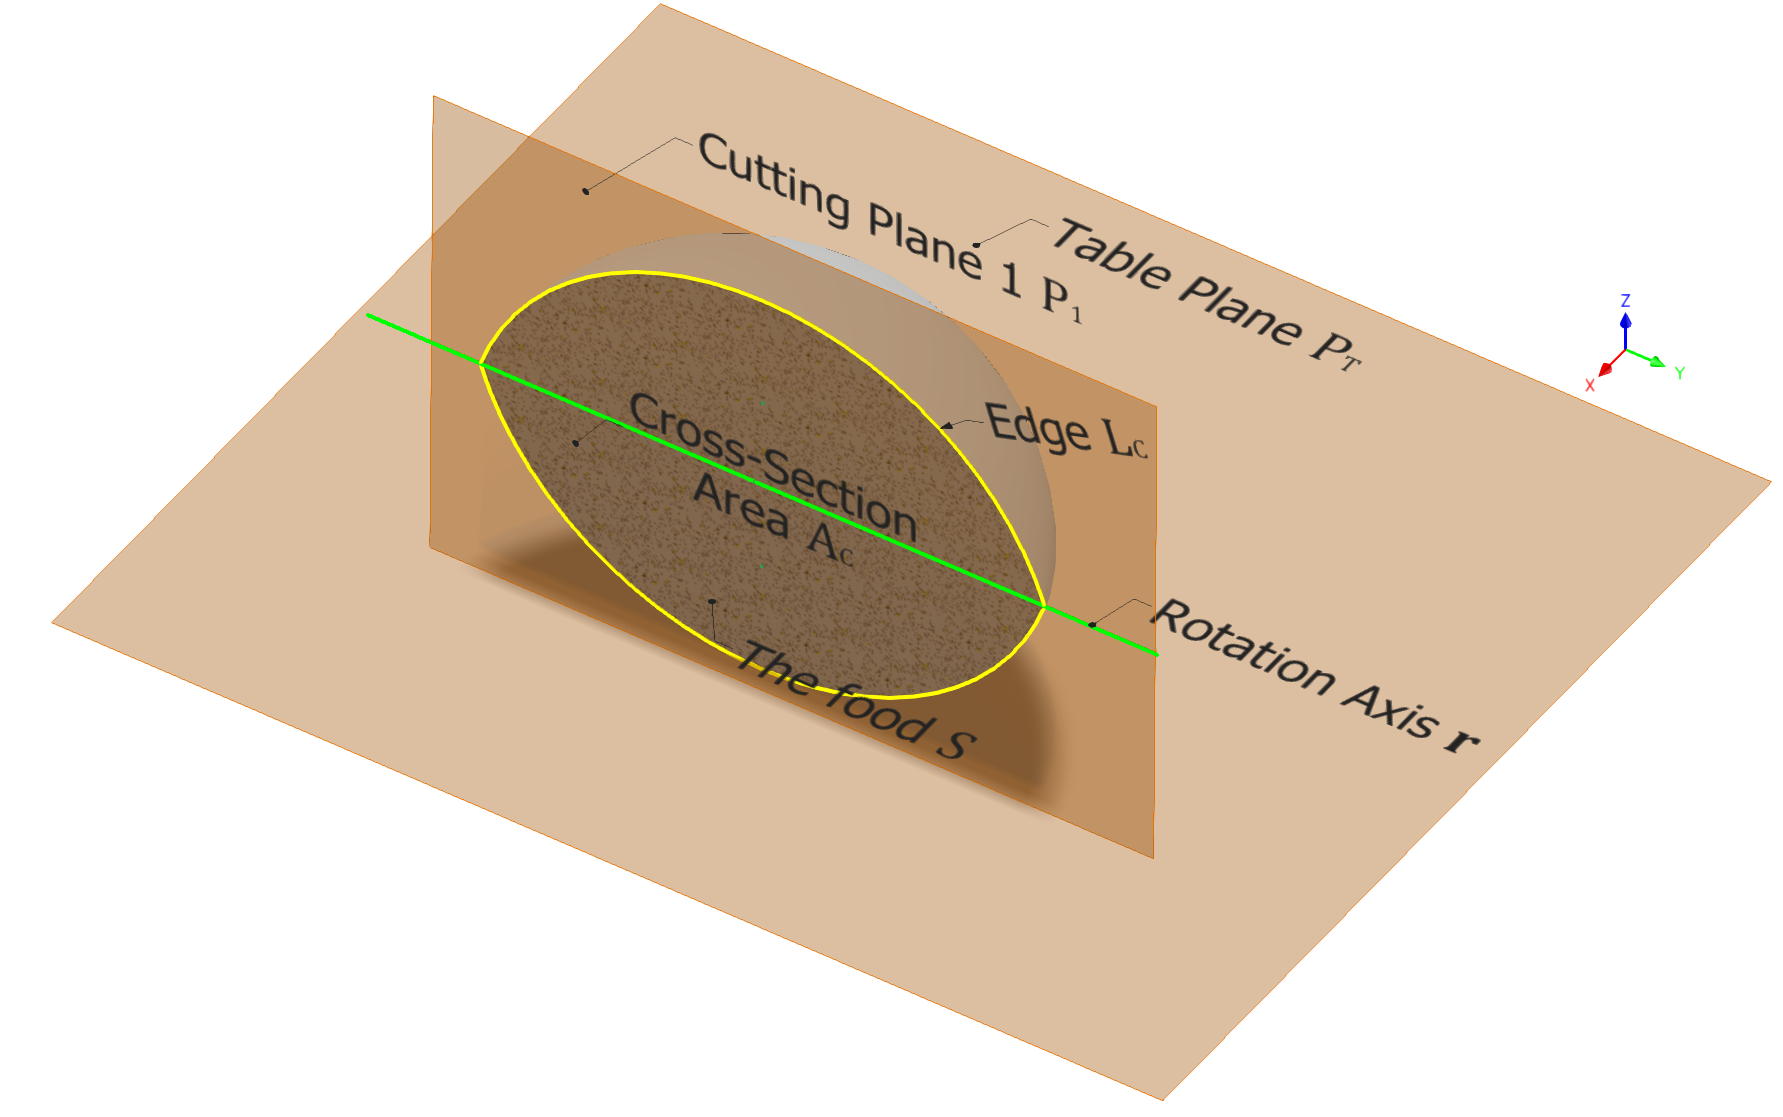
\includegraphics[width=1\textwidth]{fig/chp_peeling/Trajectory_cutting.png}
    	\caption{The cross-section area $\mathrm{A_c}$ that is cut by the cutting plane 1 $\mathcal{P}_\mathrm{c1}$. The yellow line $L_\mathrm{c}$ is the edge of the cross-section area.}
    	\label{fig:peeling_trajectory.sub1}
    \end{subfigure}
    \begin{subfigure}[t]{.45\textwidth}
    	\centering
    	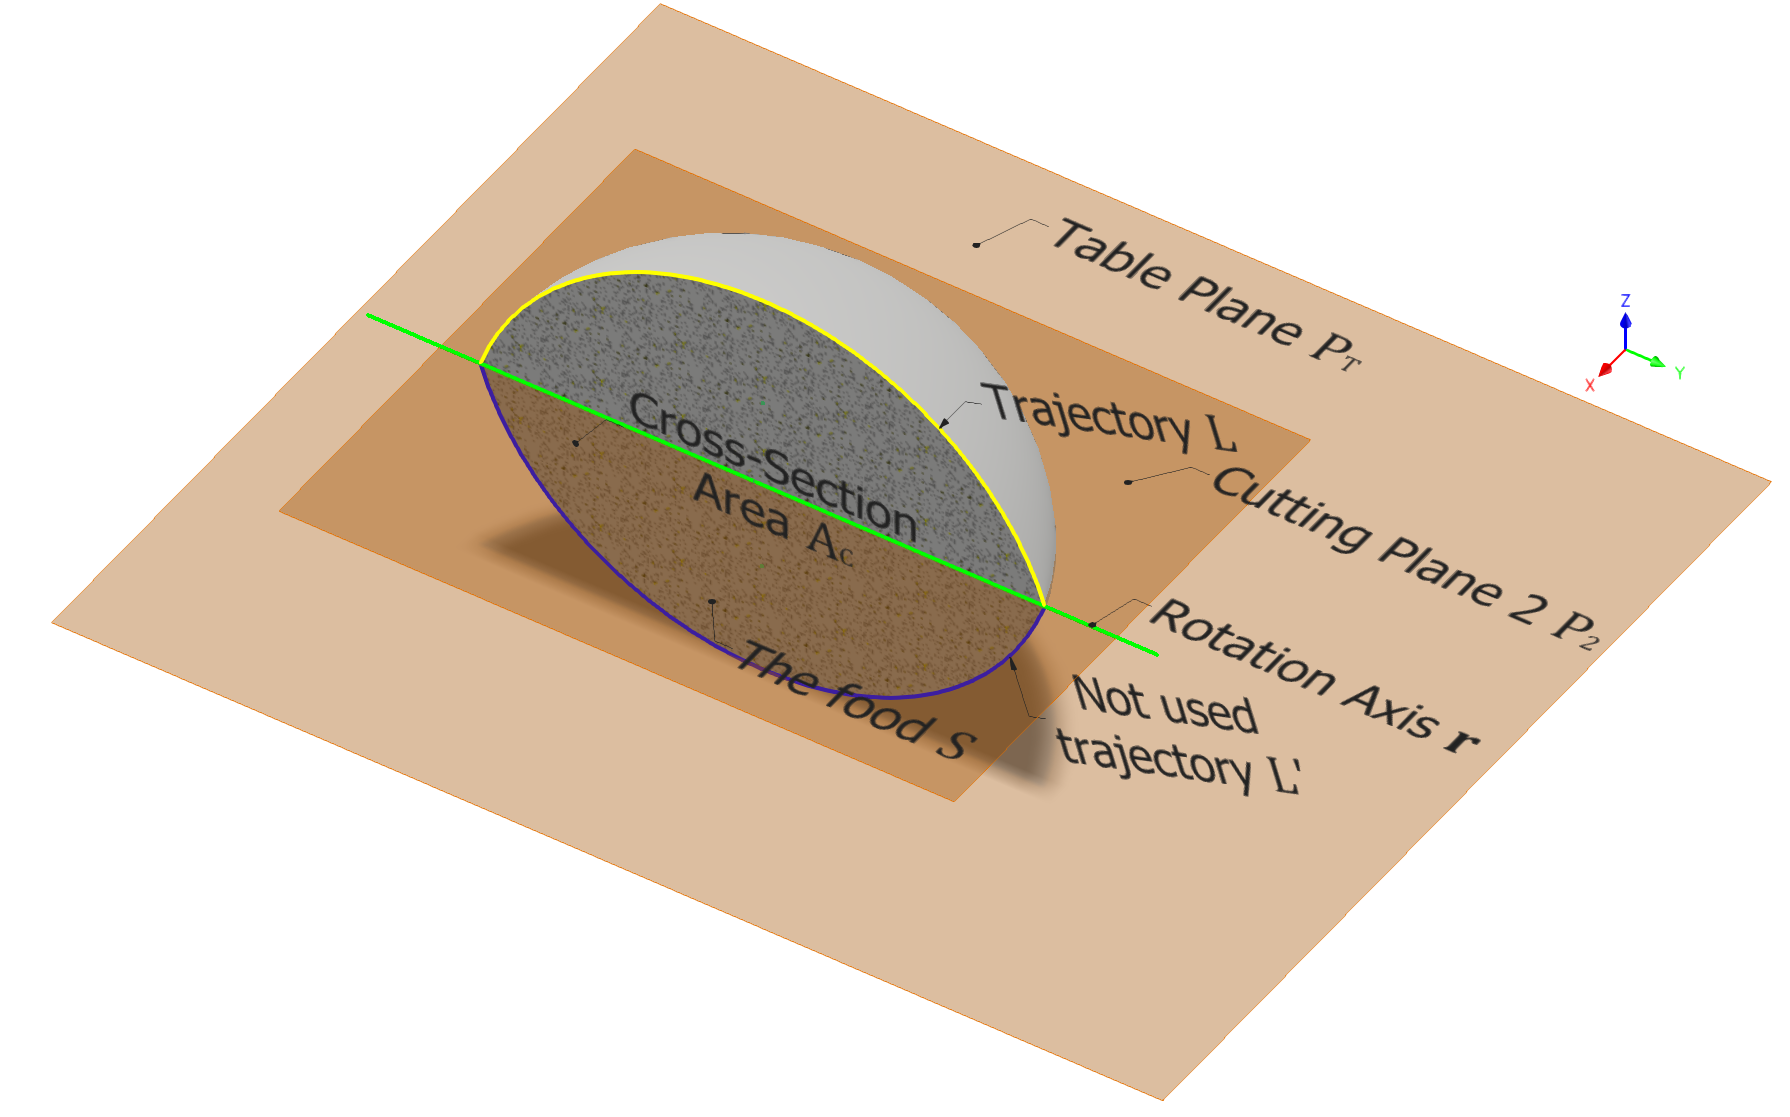
\includegraphics[width=1\textwidth]{fig/chp_peeling/Trajectory.png}
    	\caption{The result of creating the reference trajectory. The yellow line is the final trajectory $L$. The blue line $L'$ (bottom side of the food) is the trajectory that is not used.}
    	\label{fig:peeling_trajectory.sub2}
    \end{subfigure}
    \caption{The gray object is the shape of the food $\mathrm{S}$, which we is subject to peel. The largest plane with orange color is the table plane $\mathcal{P}_T$. The small plane on the left side of the images with orange color, perpendicular to the table plane, is the cutting plane 1 $\mathcal{P}_\mathrm{c1}$. The small plane on the right side of the images with orange color, parallel to the table plane, is the cutting plane 2 $\mathcal{P}_\mathrm{c2}$. The green line is the rotation axis $\mathbf{v_\mathrm{rot}}$ that is determined by human}
    \label{fig:peeling_trajectory}
\end{figure}


以上の処理をまとめると，軌跡抽出の手順は以下の通りである．

\begin{enumerate}
  \item $\mathcal{P}_{c1}$ を，$\mathbf{v}_{\mathrm{rot}}$ を含み，$\mathcal{P}_T$ に垂直な平面として定義する．
  \item $P_{\mathrm{all}}$ から，$\mathcal{P}_{c1}$ への距離が閾値0.3\,mm以内の点を抽出し，断面輪郭 $L_c$ とする．
  \item 式(\ref{eq:peeling_cut_plane_2})により $\mathcal{P}_{c2}$ の法線 $\mathbf{n}_{c2}$ を決定する．
  \item 式(\ref{eq:peeling_point_removal})により $L_c$ から下側部分を除去し，到達可能軌跡 $L$（点群 $P_L$）を得る．
\end{enumerate}

このようにして得られた基準軌跡 $L$ は，食材の回転軸を含む断面輪郭のうち，ロボットアームがピーラーを安全に到達させられる上半分の曲線となる．
本節では基準軌跡 $L$ の生成に焦点を当て，点群の取得，合成，平滑化，および法線推定の詳細は第3章で扱っているため，ここでは繰り返さない．

\subsection{法線による軌跡分割}
\label{sec:peeling_trajectory_segmentation}

抽出された基準軌跡 $L$ は，食材表面の曲率に従う3次元曲線である．
一方，ピーラーの刃は食材表面に対して受動的に回転できる構造を有しているため，ピーラーの持ち手（ハンドル）の姿勢によらず，刃先は自動的に表面に接する方向をとることができる．
この性質により，曲線全体の厳密な追跡は不要であり，軌跡を複数の直線セグメントに分割して逐次実行することが可能となる．
なお，実行時には力覚フィードバックが併用されるため，実際のロボットの移動経路は厳密な直線にはならない．

$P_L$ 上の点を実行順に $\mathbf{p}_1, \mathbf{p}_2, \ldots, \mathbf{p}_N$，対応する法線を $\mathbf{n}_1, \mathbf{n}_2, \ldots, \mathbf{n}_N$ とする．
ここで，点群の実行順への並べ替えは以下のように行う．
まず，$P_L$ の中で $z$ 座標が最大となる点を基準点とする．
基準点よりも右側の点群は，$z$ 座標が最小の点を始点として $z$ 座標の小さい順に並べる．
左側の点群は，基準点を始点として $z$ 座標の大きい順に並べる．
最後に，左右の点列を結合することで，軌跡に沿った順序の点列を得る．

軌跡分割の処理は，以下の手順で行う．

まず，軌跡 $L$ の先端の点 $\mathbf{p}_1$ を現在のセグメントの開始点 $\mathbf{p}_{\mathrm{st}}$ とし，その法線 $\mathbf{n}_1$ を参照法線 $\mathbf{n}_{\mathrm{ref}}$ とする．
次に，点の順番に走査し，各点 $\mathbf{p}_n$ の法線 $\mathbf{n}_n$ と $\mathbf{n}_{\mathrm{ref}}$ のなす角$\theta_n$を計算する．

% \[
% \theta_n = \arccos\left(\frac{\mathbf{n}_n \cdot \mathbf{n}_{\mathrm{ref}}}{\|\mathbf{n}_n\| \cdot \|\mathbf{n}_{\mathrm{ref}}\|}\right)
% \]

このなす角の角度 $\theta_n$ が閾値 $\theta_{\mathrm{th}}$ を超えた場合，$\mathbf{p}_{\mathrm{st}}$ から $\mathbf{p}_{n-1}$ までを一つのセグメント $s_j$ とする．
そして，$\mathbf{p}_n$ を新しいセグメントの開始点 $\mathbf{p}_{\mathrm{st}}$ に設定し，同様の処理を軌跡の終端まで反復する．

今回の実験では，$\theta_{\mathrm{th}} = 30^\circ$ を閾値として用いた．
各セグメント $s_j$ に対して，セグメント内の全点の法線ベクトルを平均したものを $\mathbf{a}_j$ とし，これを当該セグメントにおけるピーラー姿勢の参照方向とする．

処理手順は以下の通りである．

\begin{enumerate}
  \item 基準軌跡 $L$ 上の点群 $P_L$ を実行順に並べる．
  \item 先端の点 $\mathbf{p}_1$ をセグメント開始点 $\mathbf{p}_{\mathrm{st}}$，その法線を $\mathbf{n}_{\mathrm{ref}}$ とする．
  \item 点列に沿って各点 $\mathbf{p}_n$ の法線 $\mathbf{n}_n$ と $\mathbf{n}_{\mathrm{ref}}$ の角度差 $\theta_n$ を計算する．
  \item $\theta_n > \theta_{\mathrm{th}}$ を満たした場合，$\mathbf{p}_{\mathrm{st}}$ から $\mathbf{p}_{n-1}$ までを一つのセグメント $s_j$ とする．
  \item $\mathbf{p}_n$ を新たな $\mathbf{p}_{\mathrm{st}}$ とし，ステップ3〜4を軌跡終端まで反復する．
  \item 得られた各セグメント $s_j$ の平均法線 $\mathbf{a}_j$ をピーラー姿勢決定に用いる．
\end{enumerate}

この軌跡分割により，曲率の大きな食材（例：りんご）では多くのセグメントに分割され，曲率の小さな食材（例：きゅうり，なす）では少数のセグメントとなる．
この適応的な分割が，食材形状の多様性に対する本手法の幾何学的適応能力の一端を担っている．

\subsection{非皮領域境界に基づく回転角の計算}
\label{sec:peeling_rotation_calc}

一回皮むき動作の後，次に剥くべき領域をピーラー側へ向けるためには，食材を適切な角度だけ回転させる必要がある．
仮定より，回転操作は固定された回転軸 $\mathbf{v}_{\mathrm{rot}}$ 周りのみに行われるが，その回転角は皮むきの度に適切に決定されなければならない．
回転角が大きすぎると剥き残しが生じ，小さすぎると既剥き領域を重複して剥くことになり作業効率が低下する．
そこで，一回皮むき動作で実際に非皮領域の境界を検出し，その幾何情報から次回の回転角を計算する手法をとる．

\subsubsection{非皮領域の抽出}

一回皮むき動作の後，ピーラー側の腕を食材の上方へ移動させ，RGB-Dカメラにより食材上面のRGB点群（以下，元RGB点群と呼ぶ）を取得する．
この元RGB点群から，第3章で述べた共通処理を適用し，食材表面のRGB点群 $P_{\mathrm{all}}$ を得る．
さらに，各点の法線ベクトルを計算する．

次に，$P_{\mathrm{all}}$ の各点の色情報をRGB色空間からHSV色空間に変換し，事前に定義された非皮領域のHSV範囲に基づいて，非皮領域の点群を抽出する．
この色範囲は人間が事前に指定する．
抽出された非皮領域点群に対してクラスタリングを適用し，最大クラスタを非皮領域 $P_{\mathrm{cluster}}$ とする．
各食材の非皮領域抽出に用いるHSV範囲の例を表\ref{tab:peeling_hsv_range}に示す．

\begin{table}[ht]
  \centering
  \caption{The HSV color range of the peeled area extraction for each food}
  \label{tab:peeling_hsv_range}
  \begin{tabular}{@{}lccc@{}}
    \toprule
    Food & H [0, 180] & S [0, 256] & V [0, 256] \\
    \midrule
    Apple & [10, 156] & --- & --- \\
    Cucumber & [30, 60] & [30, 256] & [30, 256] \\
    Eggplant & [0, 125], [155, 180] & [60, 256] & --- \\
    Potato & [20, 25] & [64, 112] & [221, 256] \\
    \bottomrule
  \end{tabular}
\end{table}

なお，にんじんのように皮と中身の色差が小さい食材では，HSV色空間による非皮領域の識別が困難である．
このような場合には，回転角計算によらず，固定回転角を用いる代替手法を適用する（4.3.3項参照）．

\subsubsection{境界の検出と回転角の計算}

非皮領域点群 $P_{\mathrm{cluster}}$ から，$x$ 座標と $z$ 座標がともに最大となる点 $\mathbf{p}_{\mathrm{pe}}$ を抽出する．
この点 $\mathbf{p}_{\mathrm{pe}}$ の $x$ 座標を $X_{\mathrm{pe}}$ とする．
次に，{元のRGB点群 $P_{\mathrm{all}}$}（非皮領域のみを抽出する前の点群）から，$x$ 座標が $[X_{\mathrm{pe}}, X_{\mathrm{pe}} + d]$ の範囲に含まれる点群を抽出する．
これらを非皮領域の境界点群 $L_p$ とする．
今回の実験では，$d = 1$\,mm とした．

境界点群 $L_p$ の各点の法線ベクトル $\mathbf{n}_{\mathrm{pe}}$ を用いて，平均法線 $\mathbf{n}_{\mathrm{avg}}$ を以下の式で計算する．

\begin{equation}
  \mathbf{n}_{\mathrm{avg}} = \frac{1}{N_{\mathrm{pe}}} \sum \mathbf{n}_{\mathrm{pe}}
  \label{eq:peeling_avg_normal}
\end{equation}

ここで，$N_{\mathrm{pe}}$ は境界近傍で用いた法線の数である．

次に，食材座標系を設定する．
食材座標系の $Z$ 軸（鉛直上向き）方向の単位ベクトルを基準ベクトル $\mathbf{v}_{\mathrm{ref}}$ とする．
この基準ベクトル $\mathbf{v}_{\mathrm{ref}}$ と平均法線 $\mathbf{n}_{\mathrm{avg}}$ のなす角を，次回の食材回転角 $\alpha$ として用いる．


処理手順は以下の通りである．

\begin{enumerate}
  \item 一回皮むき動作の後，食材上面の元RGB点群 $P_{\mathrm{all}}$ を取得し，各点の法線を計算する．
  \item $P_{\mathrm{all}}$ をHSV色空間に変換し，事前定義された色範囲でフィルタリングして非皮領域点群 $P_{\mathrm{cluster}}$ を得る．
  \item $P_{\mathrm{cluster}}$ から，$x$ 座標と $z$ 座標がともに最大となる点 $\mathbf{p}_{\mathrm{pe}}$ を抽出する．
  \item $\mathbf{p}_{\mathrm{pe}}$ の $x$ 座標 $X_{\mathrm{pe}}$ を基準に，{元のRGB点群 $P_{\mathrm{all}}$} から $x$ 座標が $[X_{\mathrm{pe}}, X_{\mathrm{pe}} + d]$ の範囲の点群を抽出し，境界点群 $L_p$ とする．
  \item $L_p$ 近傍の法線を式(\ref{eq:peeling_avg_normal})により平均し，$\mathbf{n}_{\mathrm{avg}}$ を得る．
  \item $\mathbf{n}_{\mathrm{avg}}$ と $\mathbf{v}_{\mathrm{ref}}$ のなす角 $\alpha$ を回転角として求める．
\end{enumerate}

この回転角計算は，非皮領域の境界を法線情報から定量化し，次の皮むき位置を決定する「幾何学的な分析」の一部として位置づけられる．
食材の多様な曲率に対しても，境界近傍の法線平均を用いることで，局所的な形状変動に安定な回転角が得られる．

\section{皮むき動作計画・制御}
\label{sec:peeling_phase_motion}

本節では，4.2で得られた幾何情報を用いて，実際のロボット動作を生成し，実行中の接触力を制御する方法を述べる．
具体的には，一回皮むき動作の計画，接触力フィードバック制御，食材回転操作，および反復実行と終了判定を扱う．
ここでは，幾何学的な分析で得られた軌跡・法線情報を動作指令へ変換する「動作生成」の段階と，実行中に力覚情報を用いて接触状態を維持する「制御」の段階が統合される．

\subsection{一回皮むき動作の計画}
\label{sec:peeling_one_peel_motion}

一回皮むき動作では，基準軌跡 $L$ を分割して得られた各セグメント $s_j$ に対して，ピーラーの接近動作，皮むき動作，離脱動作を生成する．

\ref{sec:peeling_trajectory_segmentation}で述べたように，ピーラーの刃は食材表面に対して受動的に回転できるため，ハンドルの姿勢によらず刃先が自動的に表面に接する．
したがって，曲線全体を厳密に追跡する必要はなく，各セグメント $s_j$ を直線軌跡として扱うことができる．

各セグメント $s_j$ は，始点 $\mathbf{p}_{\mathrm{st},j}$ と終点 $\mathbf{p}_{\mathrm{end},j}$ をもつ．
ピーラーの刃先位置は，この始点から終点へ向かって移動する．
ピーラーの姿勢は，セグメント内の平均法線 $\mathbf{a}_j$ に基づいて決定する．
具体的には，ピーラーのツール座標系の $z$ 軸方向（刃先を食材に押し付ける方向）が平均法線 $\mathbf{a}_j$ と平行になるように姿勢を設定する．

処理手順は以下の通りである．

\begin{enumerate}
  \item 分割済み軌跡 $s_1, s_2, \ldots, s_M$ を入力する．
  \item 各セグメント $s_j$ の始点 $\mathbf{p}_{\mathrm{st},j}$ と終点 $\mathbf{p}_{\mathrm{end},j}$ を求める．
  \item セグメント $s_j$ の平均法線 $\mathbf{a}_j$ から，ピーラー姿勢を決定する．
  \item セグメント開始点の手前（食材表面から法線方向に一定距離離れた位置）に接近点を設定する．
  \item 接近点から始点へ移動し，ピーラー刃先を食材表面に接触させる．
  \item 始点から終点まで，力覚フィードバック制御（4.3.2項）を用いながらピーラーを移動させる．
  \item 終点到達後，法線方向に沿って離脱点へ移動し，次のセグメントへ移る．
  \item 全セグメント $s_1$ から $s_M$ まで，ステップ2〜7を繰り返す．
\end{enumerate}

このように，一回皮むき動作は，幾何軌跡をそのまま再生するのではなく，実機で安定に実行できるセグメント列として計画される．
各セグメントは独立した直線動作として扱われるため，セグメント間での位置誤差の累積が回避される利点がある．

\subsection{接触力フィードバック制御}
\label{sec:peeling_force_feedback}

3D点群モデルから生成した基準軌跡 $L$ は，食材の表面上の軌跡である．
しかし，実際に皮を剥くためには，ピーラーの刃先を食材表面に一定の力で押し付け，表面からわずかに内側へ切り込ませる必要がある．
単なる軌跡追跡では皮むきが成立しない理由として，以下の二つを挙げている．

\begin{enumerate}
  \item 事前生成された軌跡は食材の表面情報から得られたものであるが，皮むき動作では刃先を表面よりわずかに「内側」に入れる必要がある．そのため，表面軌跡をそのまま追跡してもピーラーは空振りする．
  \item 仮に軌跡を表面より内側にオフセットしたとしても，点群計測には不可避の誤差が含まれるため，位置制御のみではピーラーが食材表面から離れたり，逆に過大な力で押し込みすぎたりする可能性がある．
\end{enumerate}

そこで，本研究では幾何軌跡に力覚フィードバックを重ね，接触力を能動的に維持する制御手法を採用する．
ピーラーの刃には切り込み深さを制限するリミッターが備わっているため，接触力の維持さえできれば，適切な深さの皮むきが実現される．

\subsubsection{制御の基本構造}

力覚フィードバック制御では，接触力の方向は食材表面の法線方向と平行であるべきという前提に基づき，ピーラーのツール座標系の $z$ 軸方向（食材表面の法線方向）についてのみ力制御を行い，残りの5軸（$x$，$y$ 方向の位置および3軸周りの姿勢）については位置制御を行う．
このハイブリッド制御構造は，RaibertとCraig\cite{RaibertCraig1981Hybrid}のハイブリッド位置/力制御の考え方に基づくものであり，拘束方向（法線方向）と自由方向（接線方向）を分離して管理することを可能とする．

目標接触力を $f_c$，力覚センサの計測値を $f_s$ とし，接触力誤差 $f_e$ を以下で定義する．

\begin{equation}
  f_e = f_c - f_s
  \label{eq:peeling_force_error}
\end{equation}

この誤差 $f_e$ をゼロに収束させるように，接触方向（ツール座標系の $z$ 軸方向）の補正速度 $v_z$ を以下の式で決定する．

\begin{equation}
  v_z = a\,|f_e|\,\left(\frac{1}{1 + e^{-b f_e}} - \frac{1}{2}\right)
  \label{eq:peeling_vz}
\end{equation}

ここで，$a$ は力誤差 $f_e$ に対する感度を，$b$ は誤差がゼロ付近にある場合のデッドゾーン幅を表すパラメータである．
\begin{figure}[!t]
  \centering
  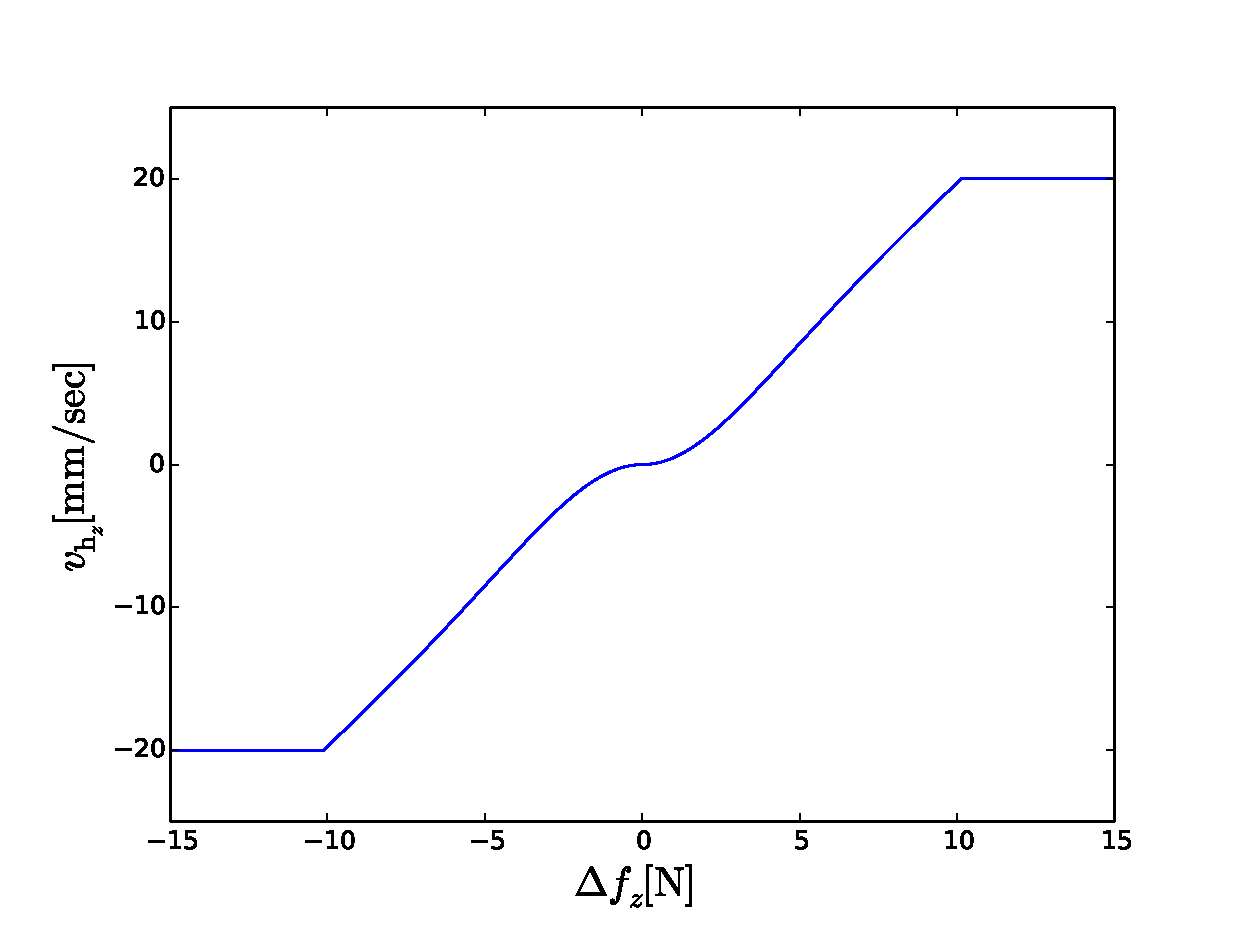
\includegraphics[width=0.75\linewidth]{fig/chp_peeling/vz_fz.eps}
  \caption{The graph of force feedback equation \ref{eq:peeling_vz}}
  \label{fig:peeling_force_feedback_graph}
\end{figure}
図\ref{fig:peeling_force_feedback_graph}で示したように，式(\ref{eq:peeling_vz})の関数の形は，基本的に $v_z$ と $f_e$ の間に線形に近い関係を持たせつつ，$f_e \approx 0$ 付近で不感帯を形成するように設計されている．
この不感帯により，微小な力計測ノイズに対する敏感な速度変動が抑制される．

\subsubsection{最低速度の設定}

実装上の課題として，式(\ref{eq:peeling_vz})では $f_e$ がゼロに近づくにつれて $v_z$ もゼロに接近するため，出力速度がロボットの動作下限を下回り，誤差が完全に収束しない現象が生じうる．
この問題を回避するため，出力速度の絶対値に最低速度 $v_{\mathrm{lim}}$ を設定する．

\begin{equation}
  v_{fz} = 
  \begin{cases}
    v_z, & \text{if}\; v_z = 0 \\[4pt]
    \mathrm{sign}(v_z)\,\max(|v_z|, v_{\mathrm{lim}}), & \text{otherwise}
  \end{cases}
  \label{eq:peeling_vz_limit}
\end{equation}

ここで，$\mathrm{sign}(v_z) = v_z / |v_z|$ は $v_z$ の符号を表す．

残りの5軸（$x$, $y$ 方向の並進および $\alpha$, $\beta$, $\gamma$ の回転）については，以下の比例制御により目標速度を生成する．

\begin{equation}
  v_i = k\,(x_{i,\mathrm{target}} - x_i),\quad i \in \{x, y, \alpha, \beta, \gamma\}
  \label{eq:peeling_position_control}
\end{equation}

ここで，$x_{i,\mathrm{target}}$ は目標位置・姿勢，$x_i$ は現在の位置・姿勢，$k$ は比例ゲインである．

\subsubsection{制御パラメータ}

今回の実験で用いられた力覚フィードバック制御のパラメータを表\ref{tab:peeling_force_params}に示す．

\begin{table}[ht]
  \centering
  \caption{The parameters of force feedback control}
  \label{tab:peeling_force_params}
  \begin{tabular}{@{}lcl@{}}
    \toprule
    Parameters & Notation & Value \\
    \midrule
    Contact force & $f_c$ & 5.0\,N \\
    Error sensitivity & $a$ & 10.0 \\
    Range of dead-zone & $b$ & 0.05 \\
    Speed min & $v_{\mathrm{lim}}$ & 0.1\,mm/s \\
    Speed max & $v_{\mathrm{max}}$ & 20.0\,mm/s \\
    \bottomrule
  \end{tabular}
\end{table}

この制御により，基準軌跡は食材形状に応じた移動方向を与え，力覚フィードバックはモデル誤差や局所的な表面凹凸を吸収する役割を担う．
すなわち，3Dモデル上の幾何学的な分析がマクロな「解」を提供し，実世界での力覚情報が微小な誤差を補償するという階層的な構造が，本手法のロバスト性の本質である．

\subsection{食材の回転操作とループ実行}
\label{sec:peeling_loop_peel_motion}

\subsubsection{食材の回転操作}

一回皮むき動作が終了し，\ref{sec:peeling_rotation_calc}で述べた手順により回転角 $\alpha$ が計算された後，食材固定側の腕が食材を回転軸 $\mathbf{v}_{\mathrm{rot}}$ 周りに角度 $\alpha$ だけ回転させる．
この回転操作により，非皮領域の隣接部がピーラー側に向き，次の一回皮むき動作の対象となる．

回転操作は，食材固定側のエンドエフェクタの回転軸周りの角度制御により実現される．
串を介して食材に回転が伝達されるため，食材と串の固定が不十分な場合には滑りが生じる可能性があるが，本実験で用いた専用エンドエフェクタ（第3章参照）により，安定した回転伝達が確保されている．

にんじんのように非皮領域の色認識が困難で，\ref{sec:peeling_rotation_calc}の回転角計算が適用できない食材については，固定回転角 $\alpha = 20^\circ$ を用いる．
この固定値は，他の食材（りんご，きゅうり，なす，じゃがいも）における回転操作回数が17〜19回の範囲に収束した実験結果に基づいて定められたものである．
すなわち，18回程度の回転で全周（$360^\circ$）をカバーするとして，$360^\circ / 18 = 20^\circ$ を固定値として採用した．

\subsubsection{終了判定}

皮むき作業の終了は，現在の食材側面における非皮領域の割合に基づいて判定する．
具体的には，非皮領域の点数 $N_{\mathrm{pe}}$ と，対象側面の全表面点数 $N_{\mathrm{side}}$ の比 $r_s$ を以下のように定義する．

\begin{equation}
  r_s = \frac{N_{\mathrm{pe}}}{N_{\mathrm{side}}}
  \label{eq:peeling_stop_ratio}
\end{equation}

この値が閾値 $r_{\mathrm{th}}$ 以上となった場合，当該側面の皮むきは十分に完了したと判断し，皮むき作業全体を終了する．

\begin{equation}
  r_s \ge r_{\mathrm{th}}
  \label{eq:peeling_stop_condition}
\end{equation}

今回の実験では，$r_{\mathrm{th}} = 0.9$ とした．

\subsubsection{反復手順}

皮むき作業の反復手順は以下の通りである．

\begin{enumerate}
  \item 食材表面点群 $P_{\mathrm{all}}$ を取得する（第3章の共通処理パイプラインによる：多視点撮影，統合，法線計算）．
  \item \ref{sec:peeling_phase_geo}節の手順により，基準軌跡 $L$ を抽出し，セグメント $s_1, s_2, \ldots, s_M$ に分割する．
  \item \ref{sec:peeling_one_peel_motion}，\ref{sec:peeling_force_feedback}項の手順により，各セグメントに沿って力覚フィードバック制御を用いながら皮むき動作を実行する（一回皮むき動作）．
  \item ピーラー側の腕を食材の上方へ移動させ，上のRGB点群を取得する．
  \item \ref{sec:peeling_rotation_calc}項の手順により，回転角 $\alpha$ を計算し，食材を回転させる（食材の回転操作）．
  \item 式(\ref{eq:peeling_stop_condition})により終了判定を行う．条件を満たさない場合は，ステップ1へ戻り，次の反復を開始する．
  \item 条件を満たした場合，皮むき作業を終了する．
\end{enumerate}

\begin{figure*}[t]
    \centering
    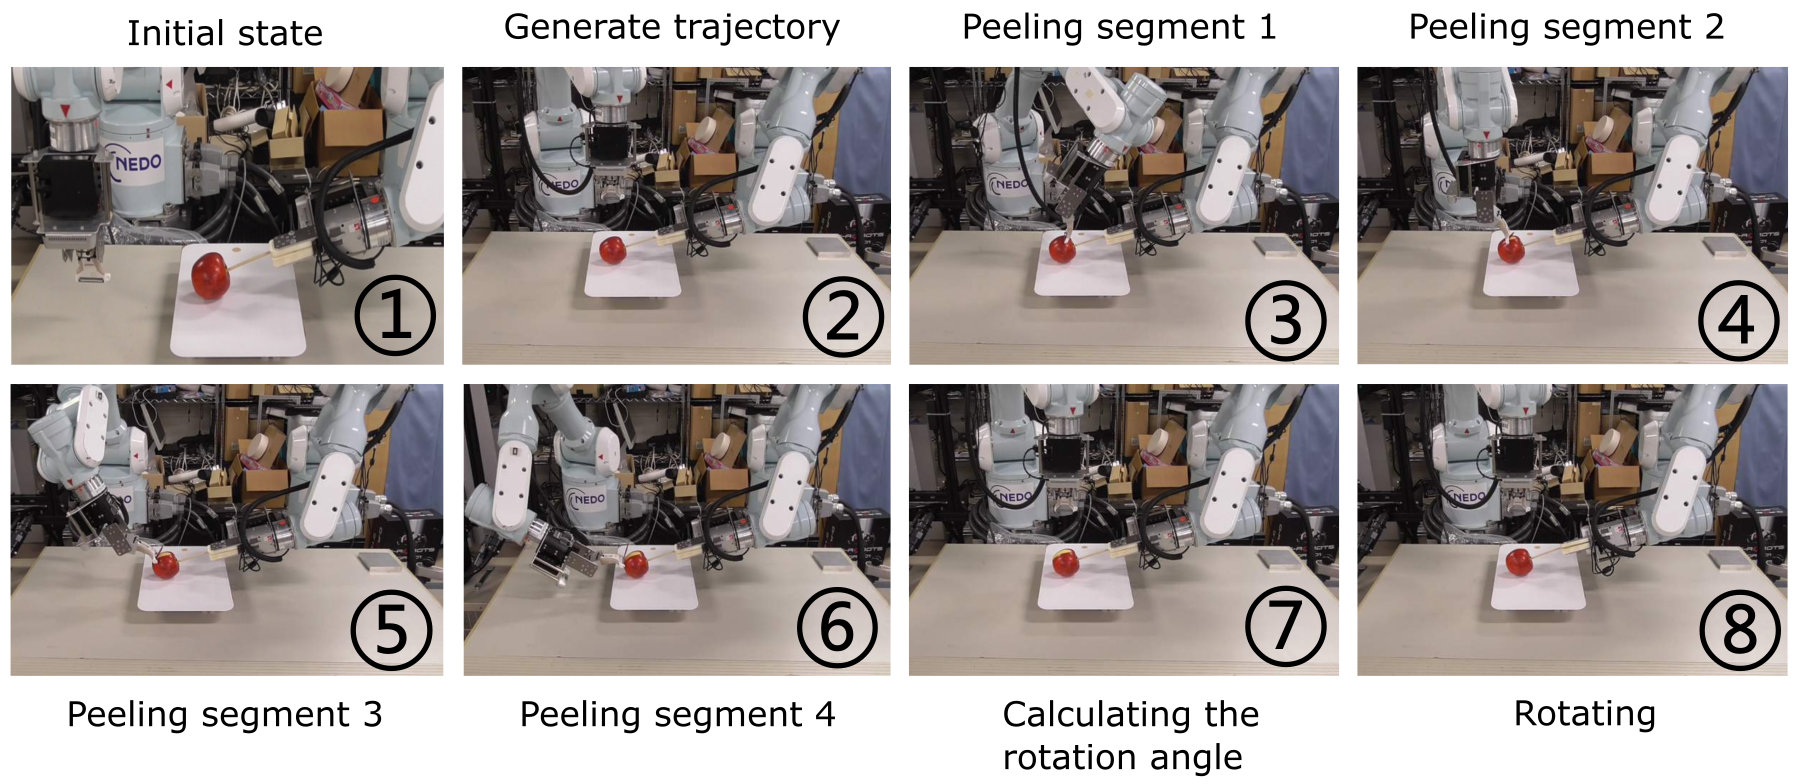
\includegraphics[width=0.95\textwidth]{fig/chp_peeling/sequence.png}
    \caption{The sequence of the proposed method. Note that if the stop condition is not satisfied, the procedure returns to step 2 while the step 8 was done.}
    \label{fig:peeling_sequence}
\end{figure*}

\section{実験}
\label{sec:peeling_phase_exp}

本節では，提案した皮むき動作生成手法を双腕ロボットシステムに実装し，複数の食材に適用する実験について述べる．

\subsection{概要}

本実験の目的は，食材表面の3D点群モデルに基づく幾何解析と，力覚フィードバック制御を組み合わせることで，形状や表面性状の異なる食材に対して皮むき動作を実現できるかを確認することである．

実験では，曲率，表面粗さ，色特徴が異なる5種類の食材を用いる．
具体的には，りんご，きゅうり，なす，じゃがいも，にんじんを対象とする．
それぞれの食材は，以下の観点から選定した．

\begin{enumerate}
  \item \textbf{りんご}：表面曲率が大きく，法線方向の変化が顕著な食材である．幾何情報に基づく軌跡生成と軌跡分割の有効性を確認する対象となる．実験では，大きさの異なる3種類（大・中・小）を各3個，計9個を用いた．りんごのサイズを表\ref{tab:peeling_apple_sizes}に示す．

  \item \textbf{きゅうり，なす}：表面曲率が比較的小さく，法線変化が緩やかな食材である．軌跡分割後のセグメント実行と接触維持の安定性を確認する対象となる．各1個を用いた．
  
  \item \textbf{じゃがいも}：表面が粗く凹凸があり，点群モデルと実表面のずれが生じやすい食材である．力覚フィードバックによる補正の有効性を確認する対象となる．1個を用いた．

  \item \textbf{にんじん}：皮と中身の色が類似しており，非皮領域の色認識が難しい食材である．RGB情報に基づく境界検出の限界を確認し，固定回転角による代替手法の有効性を検証する対象となる．1個を用いた．
\end{enumerate}

\begin{table}[ht]
  \centering
  \caption{The size of apple for experiment.}
  \label{tab:peeling_apple_sizes}
  \begin{tabular}{@{}lcc@{}}
    \toprule
    Apple & Width [mm] & Length [mm] \\
    \midrule
    Big 1 & 95.45 & 82.50 \\
    Big 2 & 95.15 & 84.40 \\
    Big 3 & 94.50 & 81.35 \\
    Medium 1 & 80.50 & 68.50 \\
    Medium 2 & 80.25 & 74.35 \\
    Medium 3 & 79.05 & 69.85 \\
    Small 1 & 53.95 & 48.85 \\
    Small 2 & 53.90 & 52.25 \\
    Small 3 & 55.05 & 46.60 \\
    \bottomrule
  \end{tabular}
\end{table}

実験では，右腕にピーラーを装着し，食材に串を刺した状態で左腕のエンドエフェクタに取り付けた．
食材の回転は，左腕の $z$ 軸周りの回転により実現した．
制御パラメータは，目標接触力 $f_c = 5.0$\,N，力誤差感度 $a = 10.0$，デッドゾーン幅 $b = 0.05$，軌跡分割閾値 $\theta_{\mathrm{th}} = 30^\circ$ とした．

ロボット本体，視覚センサ，力覚センサ，ピーラー側エンドエフェクタ，食材固定側エンドエフェクタの詳細仕様は第3章で述べているため，本節では実験目的と条件に必要な範囲に限定して記述する．

\subsection{評価指標}

皮むき結果は，非皮領域面積比 $r$ によって評価する．
実際には，面積を直接計算する代わりに点群中の点数を用いる．
これは，食材の複雑な曲面に対する面積計算を回避し，点群という本手法の基盤表現と整合的な評価を実現するためである．

評価用の点群取得にあたっては，皮むき後の食材を1視点から撮影するだけでは不可視領域のために全体の皮むき状態を把握できない．
そこで，以下の手順で評価用点群を取得する．

\begin{enumerate}
  \item 皮むき後の食材を二つに切断し，A部分・B部分とする．
  \item A部分を計測場所に置き，カメラを下方に向けて一方の側面のRGB点群 $P_A$ を取得する（点数 $N_A$）．
  \item 食材を人手で回転させ，もう一方の側面のRGB点群 $P_B$ を取得する（点数 $N_B$）．
  \item \ref{sec:peeling_rotation_calc}項と同様に，事前定義された色情報を用いて，$P_A$ から非皮領域点群 $P_{fA}$（点数 $N_{fA}$），$P_B$ から非皮領域点群 $P_{fB}$（点数 $N_{fB}$）を抽出する．
\end{enumerate}

これらの点数を用いて，皮むき率 $r$ を以下の式で計算する．

\begin{equation}
  r = \frac{N_{fA} + N_{fB}}{N_A + N_B}
  \label{eq:peeling_ratio}
\end{equation}

ここで，$r$ は非皮領域（非皮領域）の点数の，全表面点数に対する比率を表す．
すなわち，$r = 1.0$ が完全な皮むきを意味する．

\subsection{実験結果}

\begin{figure}[t]
    \centering
    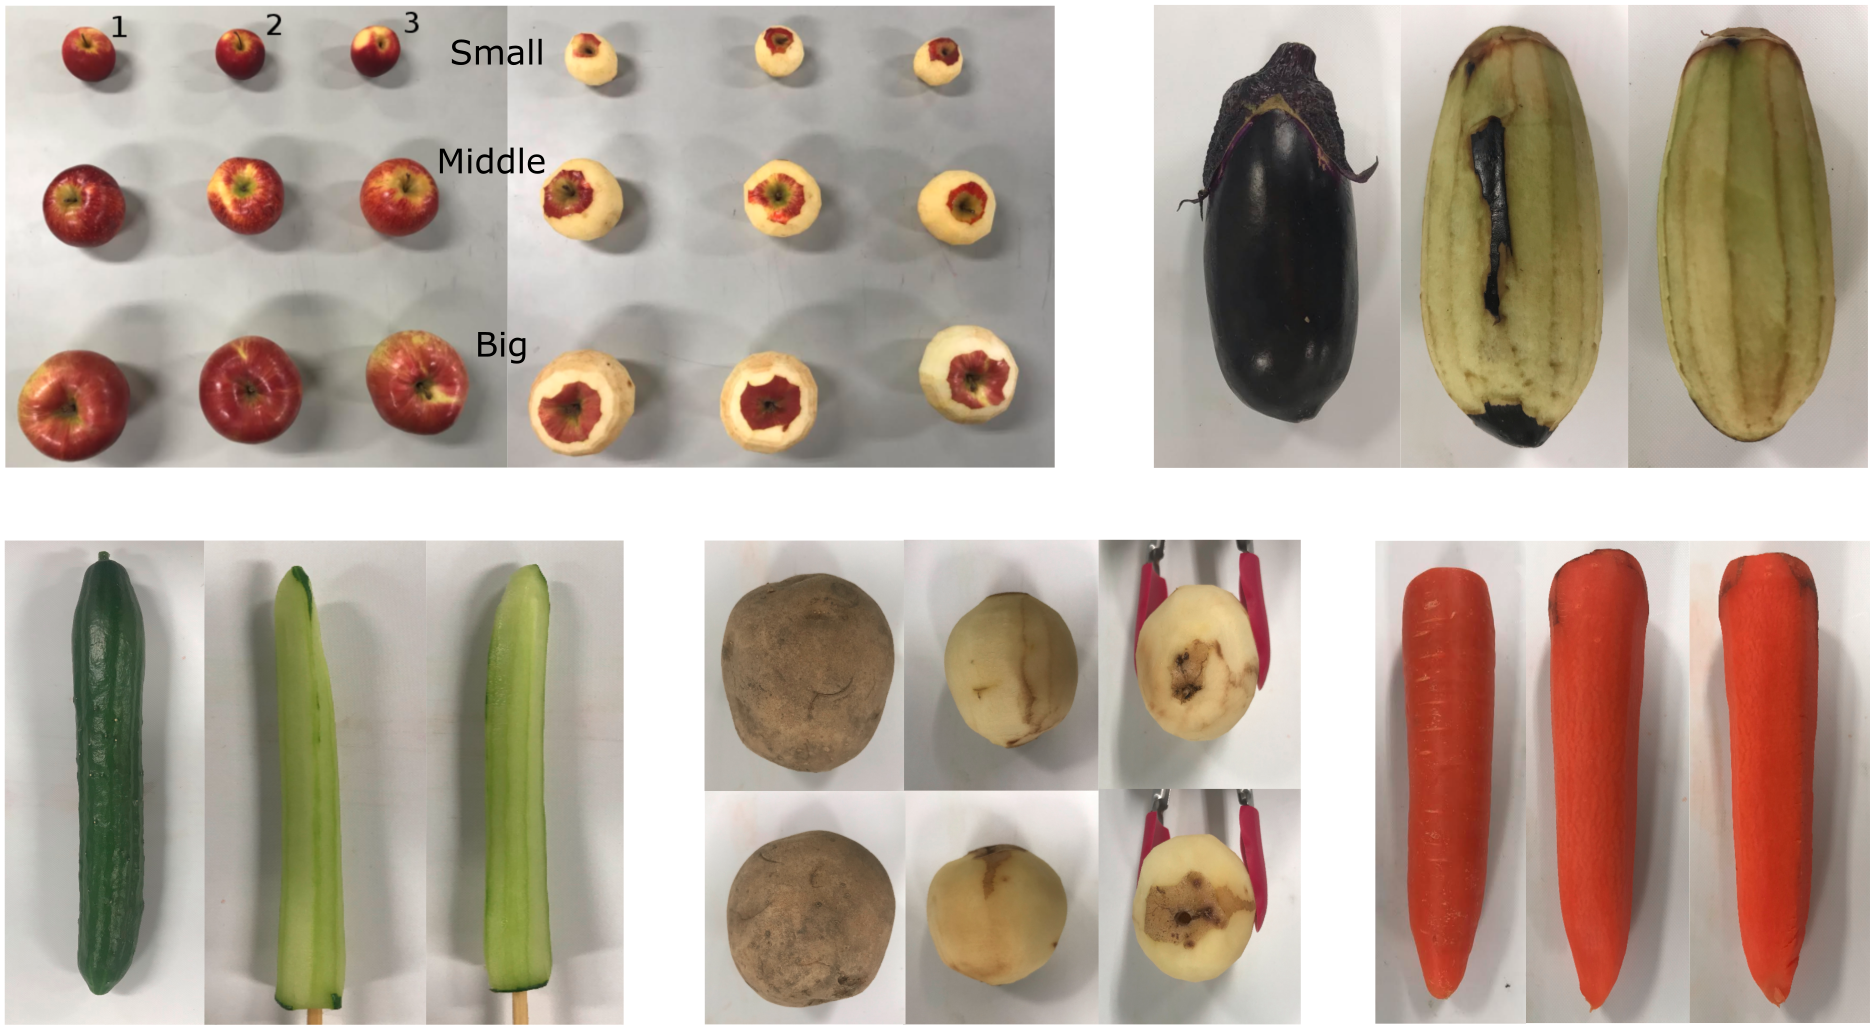
\includegraphics[width=0.7\textwidth]{fig/chp_peeling/result.png}
    \caption{The result of peeling experiment．Top left: Apples (large, medium, small); Top right: Cucumbers; Bottom left: Eggplants; Bottom middle: Potatoes; Bottom right: Carrots.}
    \label{fig:peeling_result}
\end{figure}

\subsubsection{りんご}

りんご9個（大3，中3，小3）の皮むき実験結果を図\ref{fig:peeling_result}と表\ref{tab:peeling_apple-result}に示す．

\begin{table}[t]
\centering
\caption{Peeling results for apple.}
\begin{tabular}{cccc}
	\hline
	\multirow{2}{*}{Trails} & \multicolumn{3}{c}{Ratio of the peeled area {[}\%{]}} \\ \cline{2-4} 
	& Large size     & Medium size     & Small size     \\ \hline
	1                       & 78.01          & 88.85           & 85.93          \\
	2                       & 79.83          & 84.25           & 90.93          \\
	3                       & 82.69          & 84.11           & 88.62          \\ \hline
\end{tabular}
\label{tab:peeling_apple-result}
\end{table}

りんごの結果から，全ての試行で皮むき率78\%以上を達成し，提案手法が曲率の大きな食材に対しても有効であることが確認された．
りんごの両端のくぼんだ部分は，形状的にピーラーでの皮むきが困難であり，また串に近い領域はロボットアームやエンドエフェクタとの干渉により剥きにくい．
これらの領域は，人間がりんごの皮を剥く場合にも，食べやすいサイズに切った後の段階で処理されることが多く，ピーラーで剥くことが可能な部分については提案手法で皮むきが十分に可能であることが確認された．

\subsubsection{きゅうり，なす}

きゅうり，なすの皮むき実験結果を図\ref{fig:peeling_result}と表\ref{tab:peeling_others-result}に示す．

\begin{table}[t]
\centering
\caption{Peeling results of other food. Note that the result for carrot were estimated by human eyes.}
\begin{tabular}{ccccc}
	\hline
	\multirow{2}{*}{Trails} & \multicolumn{4}{c}{Ratio of peeled area {[}\%{]}} \\ \cline{2-5} 
	& Cucumber    & Eggplant    & Potato    & Carrot    \\ \hline
	1                       & 94.31       & 90.23       & 88.72     & 95.00     \\ \hline
\end{tabular}
\label{tab:peeling_others-result}
\end{table}

きゅうり，なすのような表面の法線方向の変化が小さい食材では，りんごよりも法線のばらつきが小さいため，90\%以上の高い皮むき率が達成された．
法線変化が小さいため軌跡分割数が少なく，一つのセグメントで広範囲を安定して剥くことができたことが高い皮むき率につながったと考えられる．

なすの結果において一部の皮領域が残されたのは，終了判定のパラメータが $r_s \ge r_{\mathrm{th}} = 90\%$ と設定されており，非皮領域比率が閾値をわずかに超えた時点で作業が終了したためである．
このことから，終了判定の閾値設定が最終的な皮むき率に直接影響を与えることが確認された．

\subsubsection{じゃがいも}

じゃがいも，表面に凹凸があり，皮と中身の色が近いという二重の困難を有する食材である．
じゃがいもの結果は図\ref{fig:peeling_result}に示した．
88.72\%の皮むき率が達成されたが，芽の部分やくぼんだ部分では皮むきが十分に行われなかった．
これらの領域は，局所的に表面法線が大きく変化するため，直線セグメントによる近似では追跡しきれなかったことが原因として考えられる．

一方，表面の凹凸による点群モデルと実表面の誤差は，力覚フィードバック制御によって吸収され，全体的な接触維持は達成された．
この結果は，幾何軌跡のみでは対応できない表面粗さに対し，力覚フィードバックが有効に機能することを示している．

\subsubsection{にんじん}

にんじんは，皮と中身が同じような色をしているため，HSV色空間による非皮領域の識別が困難であった．
そのため，\ref{sec:peeling_rotation_calc}の回転角計算に代えて，固定回転角 $\alpha = 20^\circ$ を用いた．

皮むき率の評価も画像処理による自動抽出が困難であったため，目視により推定した結果，約95\%の皮むき率が得られた．
にんじんの結果は図\ref{fig:peeling_result}に示した．
固定回転角を用いた場合でも高い皮むき率が達成されたことは，$\alpha = 20^\circ$ が他の食材の回転操作回数（17〜19回）から導かれた経験的に妥当な値であることを示している．
一方で，固定回転角を用いる手法は，食材の形状や一回皮むき動作で実際に剥ける幅の変動に適応できないため，より精緻な境界認識手法の開発が今後の課題として残る．

\subsubsection{食材回転操作の回数}

各食材の皮むき作業における回転操作の回数を表\ref{tab:peeling_rotation_times}に示す．

\begin{table}[ht]
  \centering
  \caption{The times of rotation motion for each food}
  \label{tab:peeling_rotation_times}
  \begin{tabular}{@{}lcc@{}}
    \toprule
    Food &  & Rotation Times \\
    \midrule
    & Big 1 & 18 \\
    & Big 2 & 18 \\
    & Big 3 & 17 \\
    & Medium 1 & 18 \\
Apple & Medium 2 & 19 \\
    & Medium 3 & 18 \\
    & Small 1 & 18 \\
    & Small 2 & 18 \\
    & Small 3 & 17 \\
    \midrule
    Cucumber &  & 17 \\
    Eggplant &  & 18 \\
    Potato &  & 19 \\
    \bottomrule
  \end{tabular}
\end{table}

全ての食材において，回転操作回数は17〜19回の範囲に収束した．
この結果は，食材の種類や大きさによらず，一回皮むき動作で剥かれる幅と食材の全周長の比が比較的一定であることを示唆している．
この知見が，にんじんに対する固定回転角 $\alpha = 20^\circ$ の設定根拠となっている．

\subsection{考察}

考察では，結果を単に食材ごとに説明するのではなく，本章で提案した構成要素ごとに評価する．

\subsubsection{幾何情報に基づく軌跡生成の有効性}

りんごのように曲率が大きい食材では，断面輪郭に基づいて食材ごとに個別の軌跡を生成することの必要性が明確に示された．
一方，きゅうりやなすでは，法線変化が小さいため，軌跡分割後のセグメント実行が安定しやすく，94.31\%，90.23\%という高い皮むき率が達成された．

軌跡分割の閾値 $\theta_{\mathrm{th}} = 30^\circ$ は，全食材に対して共通の値で良好な結果を得たが，曲率が極端に大きい領域（例：りんごの上下端のくぼみ）では，より細かな分割が必要となる可能性がある．
適応的な閾値設定は，今後の改善方向の一つである．

\subsubsection{力覚フィードバック制御の有効性}

じゃがいものように表面が粗い食材では，点群モデルから得た軌跡と実際の接触状態の差が大きくなりやすい．
この差を力覚フィードバックが補正することで，接触を維持しながら皮むき動作を実行できた．
この結果は，本論文の「分析主導型」アプローチにおいて，幾何学的な分析（3Dモデル上の軌跡生成）と力学的制御（力覚フィードバック）の統合が有効であることを実証するものである．

なお，今回の実験では全食材に同一の制御パラメータ（$f_c = 5.0$\,N）を用いたが，食材の硬さに応じて目標接触力を調整することが，皮むき品質のさらなる向上につながると考えられる．

\subsubsection{非皮領域境界に基づく回転角計算の有効性と制限}

非皮領域を色情報により認識できる場合（りんご，きゅうり，なす），境界 $L_p$ と平均法線 $\mathbf{n}_{\mathrm{avg}}$ に基づいて次の回転角を決定する手法は有効に機能した．
特に，食材の曲率に応じて回転角が自動調整される点が，固定回転角を用いる手法に対する優位性である．

一方，にんじんのように皮と中身の色差が小さい食材では，HSV色空間による境界抽出が困難となる．
この問題に対しては，色情報以外のモダリティ（例：表面のテクスチャ変化，深層学習による領域識別）の活用が考えられる．

\subsubsection{システム上の制約と今後の課題}

串に近い領域は，ロボットアームやエンドエフェクタとの干渉により剥きにくいという構造的な制約が存在する．
これは，双腕ロボットの動作計画における到達可能性の問題であり，より多様なアプローチ方向からの皮むきや，食材把持方法の工夫が解決策として考えられる．

また，今回の実験では，皮むき作業全体の処理時間は1食材あたり約1時間を要した．
この処理時間の大部分は，点群の法線計算に費やされている．
処理時間の短縮は，実用化に向けた重要な課題である．

終了判定の閾値 $r_{\mathrm{th}} = 0.9$ によって，最大で約10\%の皮領域が残る可能性がある（なすの結果で確認された）．
この点については，終了判定基準の多角化が改善策として挙げられる．

さらに，じゃがいものような不規則形状の食材に対しては，今回の「一回皮むき＋一回回転」という反復構造では剥き残しが生じやすい．
表面法線情報に基づいて，認識された皮領域を一度に全て剥きあげた後に回転操作を実行する，といった作業構造の見直しも有効と考えられる．

\section{本章のまとめ}
\label{sec:peeling_phase_summary}

本章では，皮むき動作を対象として，第3章で得られた食材表面の3D点群モデルを入力とし，幾何情報に基づく軌跡生成と力覚フィードバック制御を統合する手法を提案・実装し，実験によりその有効性を検証した．

本章の主要な成果を以下に要約する．

\begin{enumerate}
  \item \textbf{皮むき動作の定式化}：ピーラー操作が「一回皮むき動作」と「食材の回転操作」に自然に分解されることに着目し，皮むき動作を双腕ロボット上で実装可能な形に定式化した．

  \item \textbf{幾何情報に基づく軌跡生成}：食材の回転軸を含み作業台平面に垂直な断面抽出平面 $\mathcal{P}_{c1}$ により断面輪郭 $L_c$ を抽出し，到達可能性判定平面 $\mathcal{P}_{c2}$ により下側部分を除去することで，到達可能な基準軌跡 $L$ を生成した．さらに，表面法線の変化に基づいて軌跡を複数のセグメント $s_j$ に分割し，ピーラー刃の受動的回転機能と相まって，実機での安定な直線実行を可能とした．

  \item \textbf{力覚フィードバック制御の統合}：軌跡追跡のための位置制御と，接触維持のための力制御を統合したハイブリッド制御構造を採用した．力制御には，目標接触力 $f_c$ と実測値 $f_s$ の誤差に基づく速度補正式（式(\ref{eq:peeling_vz})）を用い，最低速度 $v_{\mathrm{lim}}$ の設定により誤差収束の停滞を防止した．これにより，最終的にロバストな皮むき動作が実現された．

  \item \textbf{非皮領域に基づく回転角の計算}：RGB情報とHSV色空間を用いて非皮領域を抽出し，その境界 $L_p$ 近傍の平均法線 $\mathbf{n}_{\mathrm{avg}}$ と基準ベクトル $\mathbf{v}_{\mathrm{ref}}$ のなす角から次回の回転角 $\alpha$ を計算する手法を提案した．この手法により，食材の曲率に応じた適応的な回転角の決定が可能となった．色認識が困難な食材に対しては，固定回転角 $\alpha = 20^\circ$ による代替手法を併用した．

  \item \textbf{実機実験による検証}：りんご（9個），きゅうり，なす，じゃがいも，にんじんの合計13個の食材を用いた実機実験を実施し，全ての食材で皮むき率78\%以上を達成した．特に，きゅうり（94.31\%），なす（90.23\%），にんじん（95.00\%）では90\%以上の高い皮むき率が得られ，提案手法が形状，曲率，表面粗さ，および色特徴の異なる対象に対して適用可能であることを検証した．
\end{enumerate}

以上の結果から，3D点群モデルに基づく幾何学的な分析と力覚フィードバック制御の統合が，個体差の大きい食材の皮むき動作に対して有効なアプローチであることが示された．
本成果は，第1章で提案した「分析主導型」アプローチの具体的な実証例として位置づけられる．

次章では，対象表面へ直接工具を接触させる本章の操作から，直接把持できない液体を容器を介して操作する課題へ移る．容器の3D幾何から体積と注ぎ角度を計算することで，環境的な分析と幾何学的な分析を動作制御へ接続する．